\documentclass[10pt]{article}
%\documentclass[twocolumn]{article}
%\documentclass[onecolumn]{article}
% \usepackage{scrtime} % for \thistime (this package MUST be listed first!)
\DeclareUnicodeCharacter{0301}{\'{e}}
\usepackage{times}
\usepackage{graphicx}
\usepackage{float}
\usepackage[margin=0.75in]{geometry}
\usepackage{fancyhdr}
\usepackage{caption}
\usepackage{notoccite}
\usepackage{pgfplotstable}
\usepackage{soul} %For highlights using \hl
%\usepackage[round]{natbib}
%\setcitestyle{aysep={}} %removes the comma between the author and year in citations
%\usepackage{underscore}
\usepackage{pdfpages}
\usepackage{xcolor,colortbl}%for changing cell colour
\usepackage[normalem]{ulem}
\useunder{\uline}{\ul}{}
\usepackage{xspace}
\usepackage{booktabs}
\usepackage{capt-of}
\pagestyle{fancy}
\setlength{\headheight}{15.2pt}
\setlength{\headsep}{13 pt}
\setlength{\parindent}{28 pt}
\setlength{\parskip}{12 pt}
\pagestyle{fancyplain}
\usepackage[T1]{fontenc}
\usepackage{amsmath}
% \usepackage{color,amsmath,amssymb,amsthm,mathrsfs,amsfonts,dsfont}
\usepackage{xspace}
\usepackage{tikz-cd}
\usepackage{tikz}
\usetikzlibrary{decorations.markings}
\usetikzlibrary{calc, arrows}
\usetikzlibrary{external}
\usepackage{pgfplots}
\pgfplotsset{layers/my layer set/.define layer set={background,main,foreground}{},
        set layers=my layer set,}

\usepackage{listings}
\usepackage{xcolor}

\definecolor{codegreen}{rgb}{0,0.6,0}
\definecolor{codegray}{rgb}{0.5,0.5,0.5}
\definecolor{codepurple}{rgb}{0.58,0,0.82}
\definecolor{backcolour}{rgb}{0.95,0.95,0.92}

%for code
\lstdefinestyle{mystyle}{
	backgroundcolor=\color{backcolour},   
	commentstyle=\color{codegreen},
	keywordstyle=\color{magenta},
	numberstyle=\tiny\color{codegray},
	stringstyle=\color{codepurple},
	basicstyle=\ttfamily\footnotesize,
	breakatwhitespace=false,         
	breaklines=true,                 
	captionpos=b,                    
	keepspaces=true,                 
	numbers=left,                    
	numbersep=5pt,                  
	showspaces=false,                
	showstringspaces=false,
	showtabs=false,                  
	tabsize=2
}

\lstset{style=mystyle}
% \usetikzlibrary{pgfplots.clickable}
% \usepgfplotslibrary{clickable}
% tables
\usepackage{longtable}
\usepackage{booktabs}
\usepackage{multicol}
\usepackage{multirow}
% figs
\captionsetup[figure]{labelfont={color=blue}, font={color=black}}
%\usepackage{subfig}% http://ctan.org/pkg/subfig
\usepackage{subcaption}
%\newsubfloat{figure}% Allow sub-figures
\usepackage{caption}%lable fig caption as fig
%\captionsetup[subfigure]{labelfont=bf, justification=raggedright, labelformat=empty} %no caption label
\usepackage{stackengine} %places caption inside figure?
\captionsetup{subrefformat=empty} %when you reference the subcaption it will be (a) for example %{labelfont={color=blue}}
%\captionsetup[subfigure]{labelsep=colon}


% \usepackage{acronym}
% \usepackage{lineno}%for line numbers
%%%%%%%%%%%%%%%%%%%%%%%%%%%%%%%%%%%%%%%%%%%%%%%%%%%%%%%%%%%%%%%%%%%%%%%%%%%%%%%%
% BIBLIOGRAPHY
%%%%%%%%%%%%%%%%%%%%%%%%%%%%%%%%%%%%%%%%%%%%%%%%%%%%%%%%%%%%%%%%%%%%%%%%%%%%%%%%
\usepackage[backend=biber, giveninits=true, doi=false, isbn=false, natbib=true, url=true, eprint=false, style=authoryear-comp, sorting=nyt, sortcites=ynt, maxcitenames=2, maxbibnames=10, minbibnames = 10, uniquename=false, uniquelist=false, dashed=false]{biblatex} % can change the maxbibnames to cut long author lists to specified length followed by et al., currently set to 99.

%% bibliography for each chapter...
\DeclareFieldFormat[article,inbook,incollection,inproceedings,patent,thesis,unpublished]{title}{#1\isdot} % removes quotes around title
\renewbibmacro*{volume+number+eid}{%
	\printfield{volume}%
	%  \setunit*{\adddot}% DELETED
	\printfield{number}%
	\setunit{\space}%
	\printfield{eid}}
\DeclareFieldFormat[article]{number}{\mkbibparens{#1}}
%\renewcommand*{\newunitpunct}{\space} % remove period after date, but I like it. 
\renewbibmacro{in:}{\ifentrytype{article}{}{\printtext{\bibstring{in}\intitlepunct}}} % this remove the "In: Journal Name" from articles in the bibliography, which happens with the ynt 
\renewbibmacro*{note+pages}{%
	\printfield{note}%
	\setunit{,\space}% could add punctuation here for after volume
	\printfield{pages}%
	\newunit}    
\DefineBibliographyStrings{english}{% clears the pp from pages
	page = {\ifbibliography{}{\adddot}},
	pages = {\ifbibliography{}{\adddot}},
} 
\DeclareFieldFormat{journaltitle}{#1\isdot}
\renewcommand*{\revsdnamepunct}{}%remove comma between last name and first name
\DeclareNameAlias{sortname}{family-given}
% \DeclareNameAlias{sortname}{last-first}
\renewcommand*{\nameyeardelim}{\addspace} % remove comma in text between name and date
\addbibresource{ABC1.bib} % The filename of the bibliography
\usepackage[autostyle=true]{csquotes} % Required to generate language-dependent quotes in the bibliography
\renewrobustcmd*{\bibinitperiod}{}
% you'll have to play with the citation styles to resemble the standard in your field, or just leave them as is here. 
% or, if there is a bst file you like, just get rid of all this biblatex stuff and go back to bibtex. 
%%%%%%%%%%%%%%%%%%%%%%%%%%%%%%%%%%%%%%%%%%%%%%%%%%%%%%%%%%%%%%%%%%%%%%%%%%%%%%%%
%
% generally hyperref needs to be loaded last
\usepackage[hidelinks,colorlinks=true,linkcolor=blue,citecolor=blue,urlcolor=blue]{hyperref}
%\usepackage[hidelinks,colorlinks=false,citecolor=blue,urlcolor=darkbrown]{hyperref}
\tikzexternalize

\lhead{ABC-MCMC} %This needs to change
\rhead{Alexander Turco and GB Golding}
\title{\sc Creation of a Low Complexity Region Evolution Simulator for use in an Approximate Bayesian Computation}
\author{\sc Alexander Turco}

\providecommand{\figref}[1]{Figure \ref{#1}}  %what?
\providecommand{\tabref}[1]{(Table \ref{#1})}  %what?
\providecommand{\e}[1]{\ensuremath{\times 10^{#1}}}
\newcommand{\seg}{\texttt{Seg}\xspace}
\newcommand{\ecoli}{\mbox{\textit{E.\,coli}}\xspace}
\newcommand{\sclong}{\textit{Saccharomyces cerevisiae}\xspace}
\newcommand{\scshrt}{\mbox{\textit{S.\,cerevisiae}}\xspace}
\newcommand{\sce}{\mbox{\textit{S.\,cerevisiae}}\xspace}
\newcommand{\hslong}{\textit{Homo sapiens}\xspace}
\newcommand{\hsshrt}{\mbox{\textit{H.\,sapiens}}\xspace}
\newcommand{\hse}{\mbox{\textit{H.\,sapiens}}\xspace}
\newcommand{\celong}{\textit{Caenorhabditis elegans}\xspace}
\newcommand{\ceshrt}{\mbox{\textit{C.\,elegans}}\xspace}
\newcommand{\dmlong}{\textit{Drosophila melanogaster}\xspace}
\newcommand{\dmshrt}{\mbox{\textit{D.\,melanogaster}}\xspace}
\newcommand{\atlong}{\textit{Arabidopsis thaliana}\xspace}
\newcommand{\atshrt}{\mbox{\textit{A.\,thaliana}}\xspace}
\newcommand{\pflong}{\textit{Plasmodium falciparum}\xspace}
\newcommand{\pfshrt}{\mbox{\textit{P.\,falciparum}}\xspace}
%%%%BIBLIOGRAPHY

%Supplementary File Table Numbers:
\newcommand{\expdata}{S1\xspace}
\newcommand{\seqdata}{S2\xspace}
\newcommand{\protdata}{S3\xspace}
\newcommand{\blast}{S4\xspace}
\newcommand{\tabvar}{S5\xspace}
%Supplementary File Fig Numbers:

\newcommand{\expcor}{S1\xspace}
\newcommand{\expdistATCC}{S3\xspace}
\newcommand{\specialcell}[2][c]{%
	\begin{tabular}[#1]{@{}c@{}}#2\end{tabular}}
\newcommand{\beginsupplement}{%
	\setcounter{table}{0}
	\renewcommand{\thetable}{S\arabic{table}}%    %thetable references table counter 
	\setcounter{figure}{0}
	\renewcommand{\thefigure}{S\arabic{figure}}%
	\setcounter{equation}{0}
	\renewcommand{\theequation}{S\arabic{equation}}%

}
\renewcommand{\thesection}{}
\renewcommand{\thesubsection}{}
\renewcommand{\thesubsubsection}{}
\usepackage{setspace}
%adjust spacing
\doublespacing
\usepackage{titlesec}

\titlespacing\section{0pt}{12pt plus 2pt minus 2pt}{0pt plus 1pt minus 1pt}
\titlespacing\subsection{0pt}{12pt plus 2pt minus 2pt}{0pt plus 1pt minus 1pt}
\titlespacing\subsubsection{0pt}{12pt plus 2pt minus 2pt}{0pt plus 1pt minus 1pt}

% below 3 lines will put ALL table captions at the top...not sure if
% this is what we want but it is good enough for now

% \usepackage{float}
\floatstyle{plaintop}
\restylefloat{table}
%%%%%%%%%%%%%%%%%%%%%%%%%%%%%%%%%%%%%%%%%%%%%%%%%%%%%%%%%%%%%%%%%%%
        
        \definecolor{atomictangerine}{rgb}{1.0, 0.6, 0.4}
        \definecolor{darkbrown}{rgb}{1.0, 0.56, 0.24}
        \colorlet{darkcol}{black!30!white}
        \colorlet{lightcol}{black!10!white}
        \definecolor{txtcol}{HTML}{F40000}


%%%%%%%%%%%%%%%%%%%%%%%%%%%%%%%%%%%%%%%%%%%%%%%%%%%%%%%%%%%%%%%%%%%
\begin{document}

\widowpenalty10000
\clubpenalty10000

%\linenumbers %for line numbers
\onecolumn
%\twocolumn[  
%       \begin{@twocolumnfalse}
%               \begin{center}
                        \maketitle
%               \end{center}
%                       \bigskip

\thispagestyle{empty}
\noindent \textsuperscript{1} Department of Biology, McMaster University, Hamilton, ON, Canada

\newpage
\tableofcontents
\newpage
       
\section{Abstract} 

It has been shown that among eukaryotic proteomes, the most commonly shared peptide sequences tend to lack stable three-dimensional structures and contain low information and entropy content. These sequences, now known as low-complexity regions, lack diversity in amino acid composition, but recent research has demonstrated an important role played by these regions in a variety of cellular functions. Model-based analysis of amino acid sequences is a common approach utilized to study molecular evolution, however, due to the increasing complexity of available data, many model-based approaches have become intractable due to difficulties in calculating the likelihood function. To overcome the issue of intractability, this study employs an approximate Bayesian computation Markov chain Monte Carlo algorithm (ABC-MCMC), which utilizes a simulation step in place of calculating the likelihood function. Through the simulation of mutated protein sequences, this study aims to investigate the evolution of protein low-complexity regions by estimating parameters such as mutation and insertion/deletion rates. This work provides insight into the formation of low-complexity regions, and demonstrates the potential of using approximate Bayesian computation methods for studying evolutionary genetics. 

\bigskip
                        
%\textbf{Key Words: Low complexity, entropy, amino acid sequence,
%DNA sequence \vspace*{15pt}}
                        
                        
\newpage
%       \thispagestyle{empty}   
%       \end{@twocolumnfalse}
%
%       \thispagestyle{empty}
%       \tableofcontents
%       \newpage
%       \onehalfspacing

\section{Literature Review/Proposal}
\subsection{What are Low Complexity Regions?}
For decades, it was believed that peptide sequences which lack the ability to form stable three-dimensional structures also lack specific biological function \citep{haerty2010low}. Interestingly, among eukaryotic proteomes, the most commonly
shared peptide sequences are found to be sequences with a low information content which lack a stable three-dimensional
structure \citep{marcotte1999census, bannen2007effect, haerty2010low}. These sequences have been termed ‘low-
complexity regions’ (LCRs) due to their low information content and entropy, as well as their lack of diversity in amino acid
composition \citep{wootton1993statistics, coletta2010low}. LCRs are found in DNA as well as protein sequences and can
present in a variety of ways, all of which skew the composition of amino acids in a different manner \citep{wootton1993statistics, mier2020disentangling}. Homorepeats, direpeats, tandem repeats, and imperfect repeats are common definitions of LCRs based
on the periodicity of amino acids in a given sequence, but not every LCR is defined by a specific pattern \citep{mier2020disentangling}.Most of the time, these patterns are found to occur in non-coding regions and evolve with minimal selective pressure \citep{kruglyak2000distribution}. Further research is being done in order to uncover the function of LCRs in protein coding regions, as well as the evolutionary background of these repetitive regions \citep{huntley2006selection}. To investigate the process of LCR evolution,this study proposes an Approximate Bayesian Computation (ABC) approach which will enable the prediction of evolutionary
parameters such as mutation rates and insertion/deletion rates.

\subsection{Characteristics and Types of LCRs}
Algorithms to detect the presence of low complexity regions in a sequence are available, and continue to be improved
with further research into LCRs. \citet{wootton1993statistics} first developed an algorithm called SEG to find low complexity
regions in protein sequences using information content \citep{huntley2002simple}. Information content is a common charac-
teristic used to identify low complexity regions and in order to calculate the amount of information within a segment, the SEG
algorithm implements Shannon’s entropy \citep{wootton1993statistics,battistuzzi2016profiles}. Shannon’s entropy \citep{shannon1948mathematical} has been commonly used as a measure of complexity of a string of characters \citep{wootton1993statistics, coletta2010low, battistuzzi2016profiles}. This study will use the SEG algorithm and therefore Shannon’s entropy to assess the complexity of protein sequences. The less complex a sequence is (low variety of residues), the lower the entropy/information content of the sequence. Although LCRs are defined by their low information content, these regions have also been found to be hyper-mutable, and it is thought that throughout evolutionary history, they frequently gained and lost repeats \citep{kruglyak1998equilibrium, marcotte1999census}. In studying the \dmlong gene mastermind, which encodes a highly repetitive nuclear protein, \citet{newfeld1991interspecific} identified different patterns of evolutionary change between regions of high and low complexity. Repetitive regions were found to have a much higher rate of amino acid replacement, therefore the rate of evolution within these regions is higher than outside \citep{newfeld1991interspecific, huntley2000evolution}.

LCRs all share an overall low diversity of residues but present in unique ways as periodic or aperiodic repeats, which
take on the form of homopolymers and heteropolymers \citep{wootton1993statistics, battistuzzi2016profiles}. Homopoly-
mers/homorepeats are consecutive iterations of a single amino acid residue, and heteropolymers (direpeats, tandem repeats)
are consective iterations of more than one residue that can be found in a variety of different patterns based on periodicity
\citep{battistuzzi2016profiles, mier2020disentangling}. Microsatellites, one of the best studied types of LCRs, commonly describe regions composed of tandem repeats that are typically made from anything between one to six nucleotides \citep{ellegren2004microsatellites}. Although microsatellites normally refer to DNA sequences, it has been found that LCRs in proteins are comparable to microsatellites \citep{depristo2006abundance}. The molecular mechanisms involved in the process of evolution including slippage and unequal recombination are important for microsatellites and therefore protein LCRs as well \citep{depristo2006abundance}. A class of proteins which are related to, but slightly differ from LCRs are intrinsically disordered proteins (IDPs). IDPs are unable to form stable three dimensional structures and are characterized by low sequence complexity, biased amino acid composition, and high proportions of charged and hydrophilic residues \citep{wright2015intrinsically}. IDPs are composed of intrinsically disordered regions which are not necessarily defined by a low information content as LCRs are \citep{ dunker2002intrinsic, haerty2010low}. In this study, we propose a focus on low complexity regions.

\subsection{Why care about LCRs?}
Proteins continue to be a large area of research due to their involvement in vital cellular processes and many human
diseases. In protein sequence databases such as Swiss-Prot, the increase in the number of sequences and organisms represented
has subsequently led to a decrease in the proportion of proteins containing LCRs \citep{coletta2010low}. On top of this, there
is a lack of representation of LCRs in the protein data bank \citep{huntley2002simple}. Despite this underrepresentation
of LCRs, they are known to be associated with several human neurodegenerative diseases and are thought to serve important
biological functions \citep{huntley2006selection, coletta2010low}. It has also been found that the proteins of \textit{Plasmodium
falciparum} (the human malaria parasite) contain a high incidence of LCRs which has further highlighted the importance of both
the evolution and function of LCRs \citep{gardner2002genome, depristo2006abundance}. LCRs can appear as trinucleotide repeats which
form repeated units of three nucleotides and are a well known form of deleterious mutation in humans \citep{ross1993genes}. These
are found to be the cause of diseases including fragile X syndrome, myotonic dystrophy, spinal atrophy, muscular atrophy,
and Huntington’s disease \citep{ross1993genes}. These diseases can be broadly classified into two distinct groups, translated
polyglutamine triplet repeat diseases and untranslated triplet repeat diseases \citep{everett2004trinucleotide}. Polyglutamine triplet
repeat diseases, such as Huntington’s disease, result in the formation of protein aggregates in the cell and occur due to expanded
repeats being translated into expanded polyglutamine residues \citep{everett2004trinucleotide}. Untranslated triplet repeat diseases
such as myotonic dystrophy and fragile X syndrome differ from polyglutamine repeat diseases as they contain trinucleotide
repeats which are not translated into expansion within a mutant protein \citep{everett2004trinucleotide}.

LCRs have been associated with important biological processes such as genetic recombination, antigen diversification, and
protein-protein interactions \citep{karlin2002amino, verstrepen2005intragenic, kumari2015low}. The repetitve regions are thought
to drive recombination events which alter genes and result in phenotypic variation \citep{verstrepen2005intragenic}. In the genomes of
\textit{Haemophilus influenzae} and \textit{Neisseria meningitidis}, LCRs are abundant and cause phase variation which gives the bacteria the
ability to change their adherence patterns to host cells \citep{bayliss2001simple}. This ultimately increases the fitness of the population and allows the bacteria to evade the host response \citep{bayliss2001simple}. It was previously believed, based on structural evidence,that these hypermutable LCRs did not form stable structures but instead existed as solvent-exposed disordered coils \citep{wootton1993statistics, huntley2002simple, depristo2006abundance}. Using proteins from a non-redundant Protein Data Bank (PDB) dataset, \citet{kumari2015low} analyzed secondary structure content and surface accessibility and discovered that LCRs
can form secondary structures within proteins. More specifically, in a large majority of identified LCRs, the analysis revealed
the presence of more than one secondary structure, indicating that LCRs are found in regions where structure transition occurs
\citep{kumari2015low}. Although more work is necessary to further understand the functions of LCRs, their role in genetic
recombination, protein structure and function, and antigen diversity, highlight the importance of LCR research.

\subsection{How do LCRs Evolve?}
Although research surrounding the evolution of LCRs is lacking, there are two proposed mechanisms of microsatellite
evolution, which can be applied to many forms of LCRs. The first, polymerase slippage or slipped strand mispairing, involves
loops being formed in either the coding or template strand, which causes a misalignment of strands and results in either
the insertion or deletion of repetitive motifs \citep{levinson1987slipped, ellegren2004microsatellites}. It is believed that slipped strand mispairing is the predominant mode of mutation of LCRs, specifically in homopolymer sequences \citep{levinson1987slipped}. The second mechanism, unequal recombination, occurs when repetitive regions in homologous chromosomes do not
align properly during meiosis, which results in the repetitive region being expanded in one chromosome and contracted in
the other \citep{warren1997polyalanine, mirkin2007expandable}. In order to gain more insight into the evolutionary background of a variety of organisms, researchers have created models of events such as slippage in order to estimate mutation rate and other evolutionary parameters \citep{kruglyak2000distribution}. In a study of 10,844 parent/child allele transfers at nine short tandem repeat loci, \citet{brinkmann1998mutation} discovered 23 mutations, all of which were either gains or losses of repeats. Of the 23 mutations, 22 were due to single repeat mutations, which is why it has been common to use the stepwise mutation model of Ohta and Kimura (1973),that assumes repetitive regions expand or contract by 1 unit at a specific mutation rate \citep{brinkmann1998mutation, kruglyak2000distribution}. There are however, major drawbacks of the stepwise mutation model including that lengths can become negative, and the collection of repeat lengths in a sample will not have a stationary distribution \citep{kruglyak2000distribution}. It was thought that more complex models of LCR evolution were necessary to gain more accurate results, thus \citet{kruglyak1998equilibrium} proposed a model that incorporated length dependent slippage events. This differed from the stepwise mutation model in that the balance between slippage events and point mutations produced an equilibrium distribution of repeats \citep{kruglyak1998equilibrium}.

Models of LCR formation including replication slippage support the historical belief that LCRs evolve neutrally. More
recently, there has been increasing evidence suggesting that LCRs are also acted upon by selective pressure \citep{haerty2010low}. Kimura (1983), proposed the neutral theory of molecular evolution which suggests that selection does not play a role
in the genetic diversity within and between species, rather genetic diversity is neutral \citep{nevo2001genetic}. Evidence for the neutral evolution of LCRs relies on a large number of factors including both their lack of stable structure and function \citep{dunker2002intrinsic, haerty2010low}, and ability to frequently gain or lose repeats through replication slippage \citep{kruglyak1998equilibrium, marcotte1999census, huntley2000evolution}. Support for a selective model of LCR evolution comes from the non-random patterns of changes within LCRs, the deleterious effect of their expansion in humans \citep{karlin2002amino}, and their
enrichment in proteins involved in transcription, DNA, protein binding, reproduction, and development \citep{huntley2007evolutionary, haerty2010genome, battistuzzi2016profiles}. In a study of orthologous mouse and human genes, \citet{mularoni2007highly} found a significant negative correlation between repeat number and gene nonsynonomous substitution rate, indicating
that proteins acted upon by strong selective pressure contain a large number of repeats conserved between the two species
\citep{mularoni2007highly}. Interestingly, the study also reported a significant positive correlation between repeat size difference
and protein nonsynonymous substitution rate, demonstrating that events such as slippage and substitutions occur in proteins
which undergo neutral evolution \citep{mularoni2007highly}. It was later revealed in a study by \citet{battistuzzi2016profiles} in which 11 representative Apicomplexa genomes were analyzed, that neutral mechanisms were found to act on highly repetitive LCRs
(homopolymers) whereas selective pressures were influenced by the heterogeneity and length of the LCR \citep{battistuzzi2016profiles}. This work only begins to unravel the complexities of the evolutionary patterns associated with LCRs.

\subsection{What is an Approximate Bayesian Computation Markov chain Monte Carlo algorithm?}
When studying molecular evolution, a common practice is to use model-based analyses of sets of DNA and amino acid
sequences \citep{laurin2022jump}. This approach allows for the estimation of evolutionary genetic parameters such as
mutation rates and insertion/deletion rates \citep{wu2015estimation}. Model-based statistical inference generally revolves around
calculating the likelihood function, which represents the probability of the observed data under a chosen model \citep{sunnaaker2013approximate}. The likelihood function therefore quantifies how well the data supports both the parameter values as well as the model \citep{sunnaaker2013approximate}. However, due to an increase in the complexity and magnitude of available data, many current model-based analyses have become intractable by virtue of the likelihood function being difficult to calculate \citep{marjoram2013approximation}. Approximate Bayesian computation (ABC) methods are rooted in Bayesian statistics and have been gaining popularity in areas such as genetics, as they bypass the calculation of the likelihood function \citep{sunnaaker2013approximate}. The way in which they do this is by utilizing a simulation step in place of the calculation as a way to provide an estimate of the likelihood function \citep{marjoram2013approximation}. Since there are many ways to approach a simulation, there are many different forms of ABCs. The more popular forms include ABC rejection methods, ABC Markov chain Monte Carlo methods (ABC-MCMC), and Sequential Monte Carlo ABC methods (ABC-SMC) \citep{marjoram2013approximation}. This study proposes the use of an ABC-MCMC algorithm in order to estimate evolutionary parameters such as mutation and indel rates, and provide insight into the formation and evolution of protein LCRs.

The reason for proposing an ABC-MCMC in this study stems from the lack of a pre-existing model which explains how
insertions and deletions work. Insertions and deletions alter the landscape of a sequence, making the likelihood calculation
extremely challenging. \citet{marjoram2003markov} originally proposed the algorithm for a MCMC method without the use of
likelihoods. The algorithm first starts from a selected parameter value and proposes a move to a new parameter value based
on a proposal distribution \citep{marjoram2003markov}. Using this new parameter value, a dataset is then simulated and summary
statistics are calculated, which makes it possible to quantitatively compare differences between the simulated dataset and the
observed dataset \citep{marjoram2003markov}. If the difference between summary statistics is small, the Hastings Ratio is calculated
and the proposed parameter value can be accepted with a certain probability, then a new value is proposed and the process begins
again \citep{marjoram2003markov}. On the other hand if the difference in summary statistics between the observed and simulated
data is very large, we propose a new parameter value and begin the algorithm again \citep{marjoram2003markov, marjoram2013approximation}. The use of this algorithm has enabled the analysis of complex problems which tend to arise in the areas of population genetics, ecology, epidemiology, and systems biology \citep{sunnaaker2013approximate}. The group of \citet{liepe2010abc} have been leaders in the use of ABCs for inference of genetic networks. This is evident through the creation of a software package they created called ABC SysBio which can implement ABC algorithms in a straightforward manner \citep{liepe2010abc, marjoram2013approximation}. Prior to the year 2000, there were essentially no papers published on ABCs \citep{marjoram2013approximation}. As we enter into an era where larger and more complex data can be collected, the need for improved models is necessary, hence the large increase over the last decade in papers which mention ABC methods \citep{marjoram2013approximation}.

\subsection{How will we use an ABC-MCMC - (Oct 28 Proposal, To See New Process Refer to \hyperref[methods]{Materials and Methods})}
Using the algorithm mentioned above for an ABC-MCMC, this study aims to better understand the evolutionary back-
ground/formation of protein LCRs. An ABC-MCMC will enable the prediction of two important evolutionary parameters,
mutation rate and indel rate. There is possibilty for the estimation of other parameters which will be explored upon investi-
gating the first two. We will utilize amino acid sequences in this study, one being the SRP40 protein found in \sclong, which is extremely biased in composition. This protein sequence will act as our observed data and we will compare
this observed data to our simulated data.

In terms of a simulation, we will use C++ to first generate a random amino acid sequence of a certain length. This
randomly generated sequence will then be mutated over a number of generations in a two-step process. The first process is
to choose a random Poisson deviate with a mean that is equal to the mutation rate multiplied by the total number of sites. A
Poisson distribution is used here because mutation is a rare event and rare events can be modelled using this distribution. The
value of the Poisson deviate yields the total number of sites in the simulated sequence which should be mutated at random.
The second mutation process deals with amino acid expansion and in this case we iterate through each residue in the simulated
protein sequence and scan for repeats. If a residue is part of a repeat, we take the total length of the repeat, multiply it by the
mutation rate and use this value as the mean of a random exponential deviate. We use the exponential distribution as it models
waiting times between events. Based on the random exponential deviates assigned, we select the lowest value which represents
the residue that will change fastest, and we alter that residue to either delete or insert a repeat at that position.

Once we simulate a protein sequence for a number of generations under certain parameter values, we need to obtain a
set of summary statistics and compare the summary statistics of the observed and simulated data. We have proposed summary
statistics based off notable characteristics such as protein length, number of LCRs, and the average entropy of the LCRs. There
is the possibility for additional summary statistic characteristics upon exploration of the initially proposed characteristics. To
quantitatively compare the differences between the observed and simulated data, we propose using a distance measure between
the two vectors of summary statistics. This distance is just the norm of the vector observed-simulated. Along with this, we also
propose the use of a threshold as a way to assess how close the two datasets are. If the distance between the two vectors of
summary statistics is larger than this threshold, we can not accept the proposed parameter value and the algorithm begins again.
On the other hand, if the distance is very small, we can move forward in the algorithm and potentially accept the new parameter
value.

We intend to run the simulation under the same parameters many times and take the average of the produced summary
statistic vectors before calculating the distance between observed and simulated data. It is also worth noting that each time we
begin the algorithm again, new parameter proposals will be selected using random normal deviates. We hope to see the distance
between summary statistics being minimized upon every initial iteration of the algorithm (burn-in), and then wander around according to the distribution that was utilized. 

%\section{Introduction}

\section{Materials and Methods (mid-year stuff Jan 20)} 
\label{methods}
Custom scripts and commands utilized in this analysis can be found on \texttt{GitHub} at
\url{https://github.com/opticrom/abcmcmc-thesis4c12}.

%\sloppy For a detailed protocol, see Supplementary files on \texttt{GitHub} at
 %\url{https://github.com/JohannaEnright/LCREntropyProject/}.

\subsection{ABC-MCMC: The Algorithm}
% Here we provide the basis of the algorithm from Marjoram et al.
% Compare this to my algorithm right now

This study utilized the ABC Markov chain Monte Carlo algorithm, originally proposed by \citet{marjoram2003markov}. The algorithm begins from a randomly selected parameter value and follows the steps below.

%\begin{figure}[h]
	\begin{enumerate}
		\item If now at $\theta$, propose a move to $\theta'$ according to a proposal distribution $q(\theta, \theta')$.
		\item Simulate a dataset, $D'$ using $\theta'$.
		\item If $D' \approx D$ proceed to step 4; else, output $\theta$ and return to 1.
		\item Calculate the Hastings Ratio.
		\item Accept, and output, the new $\theta'$ with probability h. Else return to, and output, $\theta$, Go back to 1.
	\end{enumerate}
	%\label{fig:algorithm1}
	%\caption{Hello}
%\end{figure}

A custom \texttt{C++} script was written to iterate through the algorithm for a desired number of simulations. The normal distribution was used to control how new parameter values were proposed. We simulated a dataset under the newly proposed parameter value, which consisted of a randomly generated protein sequence. The simulated protein was compared to a protein of known low complexity called SRP40, which is found in the model organism \sclong. The protein sequence for SRP40 was obtained from the NCBI database. To quantitatively compare similarities between simulated and observed protein sequences, vectors of summary statistics (characteristics that describe the sequences) were created for each sequence. 

The Euclidean distance between the observed and simulated protein vectors was calculated in order to determine if the newly proposed parameter value could be accepted. If the Euclidean distance between the SRP40 vector and the vector produced using the newly proposed parameter values was smaller than the distance between the SRP40 vector and the distance calculated using the current parameter values, the newly proposed parameter values were accepted. If this distance was larger, a one sample t-test was employed to determine the probability of accepting the newly proposed parameter values.

\subsection{Parameters and Summary Statistics}
% Here we talk about which parameters and summary statistics were working with
% What is mutation rate, what is indel rate.
% I am not sure if I talk about why were using them here, I think I need to though
%My mutation rate is like point mutation rate, ask though to make sure

Two parameters were estimated in this study, mutation rate and insertion/deletion (indel) rate. Mutation rate referred to the rate at which a single amino acid in a protein sequence changed into a different amino acid. Indel rate referred to the rate at which an amino acid was deleted or inserted from a protein sequence. For the purpose of this study, to determine if the length of a repetitive region played a role in insertions, any amino acid that was inserted into the simulated protein sequence was the same unit as the previous amino acid in the sequence.

Summary statistics were utilized to capture important information about simulated and observed protein sequences in order to assess how similar the sequences were. Three summary statistics were used which included, the length of the protein sequence, the number of LCRs in the sequence, and the average entropy of the LCRs. To identify LCRs and their corresponding entropies, the \texttt{Seg} algorithm was implemented \citep{wootton1993statistics}. The following \texttt{Seg} parameters were utilized to search for LCRs in proteins; a window length of 15, a trigger segment complexity of 1.9, and an extension segment complexity of 2.2. We selected these due to previous research which demonstrated that these parameter values would better detect regions of low complexity in eukaryotes which are typically longer and contain more repetitive repeats \citep{huntley2000evolution}. Summary statistics were stored in vectors and normalized in order to prevent large values (for example the length of the protein sequence) from dominating when calculating the Euclidean distance.

\subsection{Simulation Step: Creation and Mutation of Protein Sequences}
% Bulk of methods, talk about the simulation step which involves creating proteins
% mutating proteins (indels and point mutations) and how we scan for repeats and assign deviates. the whole process, even generating deviates here
%Scale parameter is beta for exponential distribution

To bypass calculation of the likelihood function, a custom \texttt{C++} script was written to simulate the generation and mutation of protein sequences over numerous generations. Two random proteins of desired length were generated first, one that would be mutated based on the current simulation parameters, and one mutated based on the proposed simulation parameters. We generated two protein sequences 400 amino acids in length, similar to the length of the SRP40 protein in \scshrt. This simulated protein sequence was then  mutated in the following ways.

We iterated over the simulated protein sequence and assigned exponential deviates to each amino acid. We utilized the exponential distribution because it is commonly used to model waiting times between events. Mutation and indel rates served to act as the scale parameter ($\beta$), or mean of the distribution, indicative of the mean time until mutation occurs. In the case of mutation rate, the same rate was utilized across all sites, with the assumption made that repeats do not play a role in point mutation. In the case of the indel rate, we scanned for repeats, and if found, we multiplied the length of the repetitive segment by the indel rate, and utilized this new value as the scale parameter ($\beta$) for the exponential distribution.

Exponential deviates were stored in two vectors, one for deviates generated using mutation rate, and the other for deviates generated using the indel rate. We then identified a single deviate with the lowest value (based on both vectors), which represented the residue that mutated quickest. Depending on which vector the lowest deviate came from, we either altered the corresponding amino acid or inserted/deleted a repetitive amino acid. Upon mutating, deleting, or inserting an amino acid, we scanned the sequence to see if the mutation altered the landscape (inturrupted a repeat, created a repeat), and subsequently generated new deviates for the amino acids that were affected.

We ran the simulation ten times for each newly proposed parameter value and took the average of all ten vectors of summary statistics prior to calculating the distance. On each simulation, we mutated the protein sequence for 50 generations before obtaining summary statistics. We plan on testing the program in the future with various numbers of iterations.

\subsection{Normalization and Euclidean Distance Calculation}
% May be important to highlight this calculation because we use it to normalize the vectors of summary statistics before examining results.
% Could make this a weighted Euclidean Distance?
% Can I also put normalizing the vectors here?

To determine the similarity between simulated and observed protein sequences, the distance between the vectors of summary statistics was calculated by employing a Euclidean distance measure \eqref{eq:4}. Before calculating this distance, vectors of summary statistics were normalized to prevent large values (such as protein length) from dominating the distance measure.

In order to normalize all elements of the vector to be between 0 and 1, maximum and minimum values for each summary statistic were required. For the length of the simulated protein, an upper limit of 1.5x the length of the SRP40 protein, and a lower limit of 0.5x the length of the SRP40 protein were set. Due to the length of the SRP40 protein being 406 amino acids long, the upper limit was equal to 609 amino acids, and the lower limit was equal to 203 amino acids \eqref{eq:1}. In terms of the number of LCRs, the minimum value was set to 0 (no LCRs) and the maximum value was chosen based off the shortest LCR length. We selected 5 amino acids to be the length of the shortest LCR, resulting in the maximum number of LCRs being 81.2 (406/5) \eqref{eq:2}. Finally, for the average entropy of the LCRs, the minimum value was set to 0, and the maximum value was set to 4.3 (maximum entropy for amino acids). Normalization calculations are shown below.


\begin{equation}
	normalized\_length = \frac{(simulated\_protein\_length - SRP40\_length + min\_length)}{SRP40\_length}
	\label{eq:1}
\end{equation}

\begin{equation}
	normalized\_number\_LCRs = \frac{number\_LCRs}{max\_number\_LCRs}
	\label{eq:2}
\end{equation}

\begin{equation}
	normalized\_average\_entropy = \frac{average\_entropy}{max\_entropy}
	\label{eq:3}
\end{equation}

\begin{equation}
	d(P1,P2) = \sqrt{(x_2-x_1)^2 + (y_2-y_1)^2 + (z_2-z_1)^2 }
	\label{eq:4}
\end{equation}

\subsection{One Sample T-Test for Probability of Acceptance}

A one sample t-test was employed in order to assess the probability of accepting newly proposed parameter values in cases where the Euclidean distance between vectors produced using the newly proposed parameters was larger than the distance between vectors produced using the current parameter values. Essentially the t-test provided a way to assess if the newly proposed parameter values are samples of data from the same distribution. For each set of newly proposed parameter values, 10 vectors of summary statistics were produced. From these 10 vectors, 10 distances were found, and the mean and standard deviation were calculated and subsequently used in the calculation of the t-statistic \eqref{eq:5}. Vectors of t-statistics and associated probabilities were stored, and the calculated t-statistic was used to estimate a p-value by linear interpolation. 

\begin{equation}
	t = \frac{\bar{x}-\mu}{\frac{S}{\sqrt{n}}}
	\label{eq:5}
\end{equation}

\section{Results}

\subsection{Assessing the Evolution Simulator}

To be able to utilize the evolution simulator within an approximate bayesian computation, tests had to be done to ensure it was working properly. The first step in this study involved running simulations of LCR evolution for various mutation and indel rates. Simulations were run for 1000 iterations each, and on each iteration, the simulator would return the average entropy of the LCRs in the sequence, the total number of LCRs in the sequence, and the overall sequence entropy. To test the effects of each individual rate parameter, only 1 rate was adjusted while the other remained a fixed constant. \figref{fig:1} and \figref{fig:2} are the result of holding the mutation rate constant at 1, and only changing the insertion/deletion rate. It is expected that a low indel rate will lead to the formation of less LCRs and hence a higher sequence entropy. The results in \figref{fig:1} match this expectation, showing the formation of only one to two low complexity regions that are quickly removed by mutations, and a relatively unaffected maximal protein sequence entropy. 

\begin{figure}[H]
	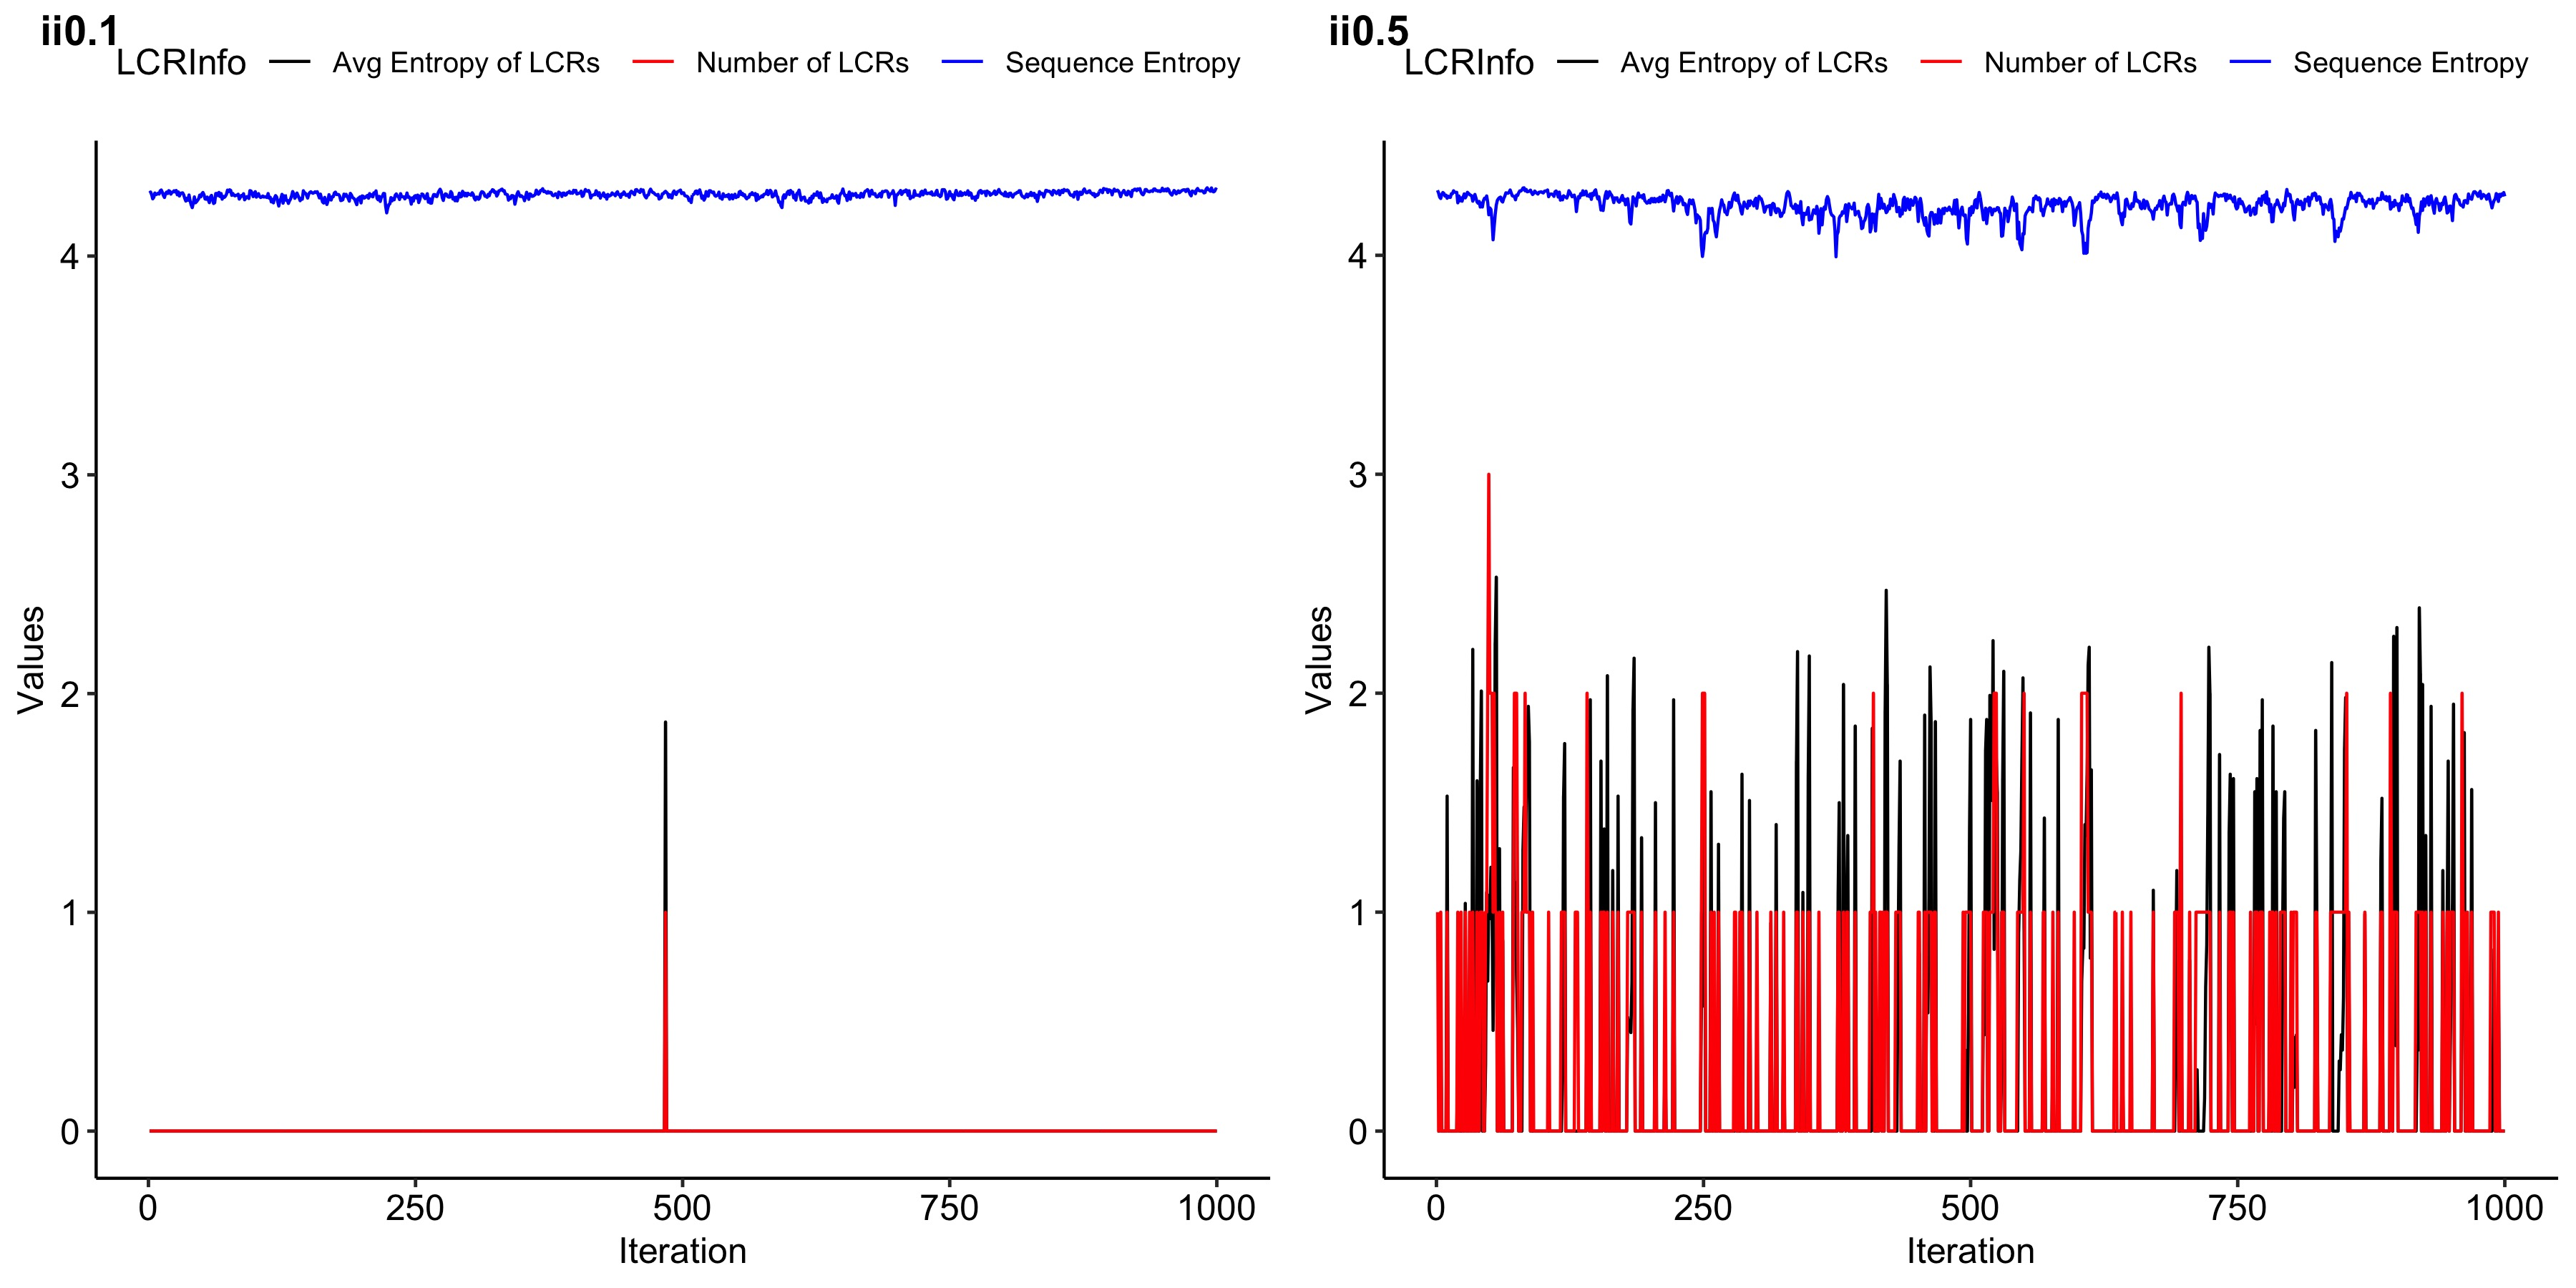
\includegraphics[width=18cm, height=10cm]{im0.01-0.1-0.5.jpeg}
	\caption{Entropy and number of LCR comparisons in a randomly generated protein sequence that has undergone simulated evolution. (Left) An indel rate of 0.1 was utilized. (RIGHT) An indel rate of 0.5 was utilized. A mutation rate of 1 was utilized for both.}
	\label{fig:1}
\end{figure}

As the indel rate is increased, it is expected that there should be more low complexity regions and hence, a lower average sequence entropy. Results in \figref{fig:2} show the formation of many more LCRs that remain in the protein sequence, possibly because mutations don't have as much of a chance swamp out the formation of low complexity regions. These results also show much more of a fluctuation in average sequence entropy compared to \figref{fig:1}, with decreases in entropy occuring where new LCRs are being formed.

\begin{figure}[H]
	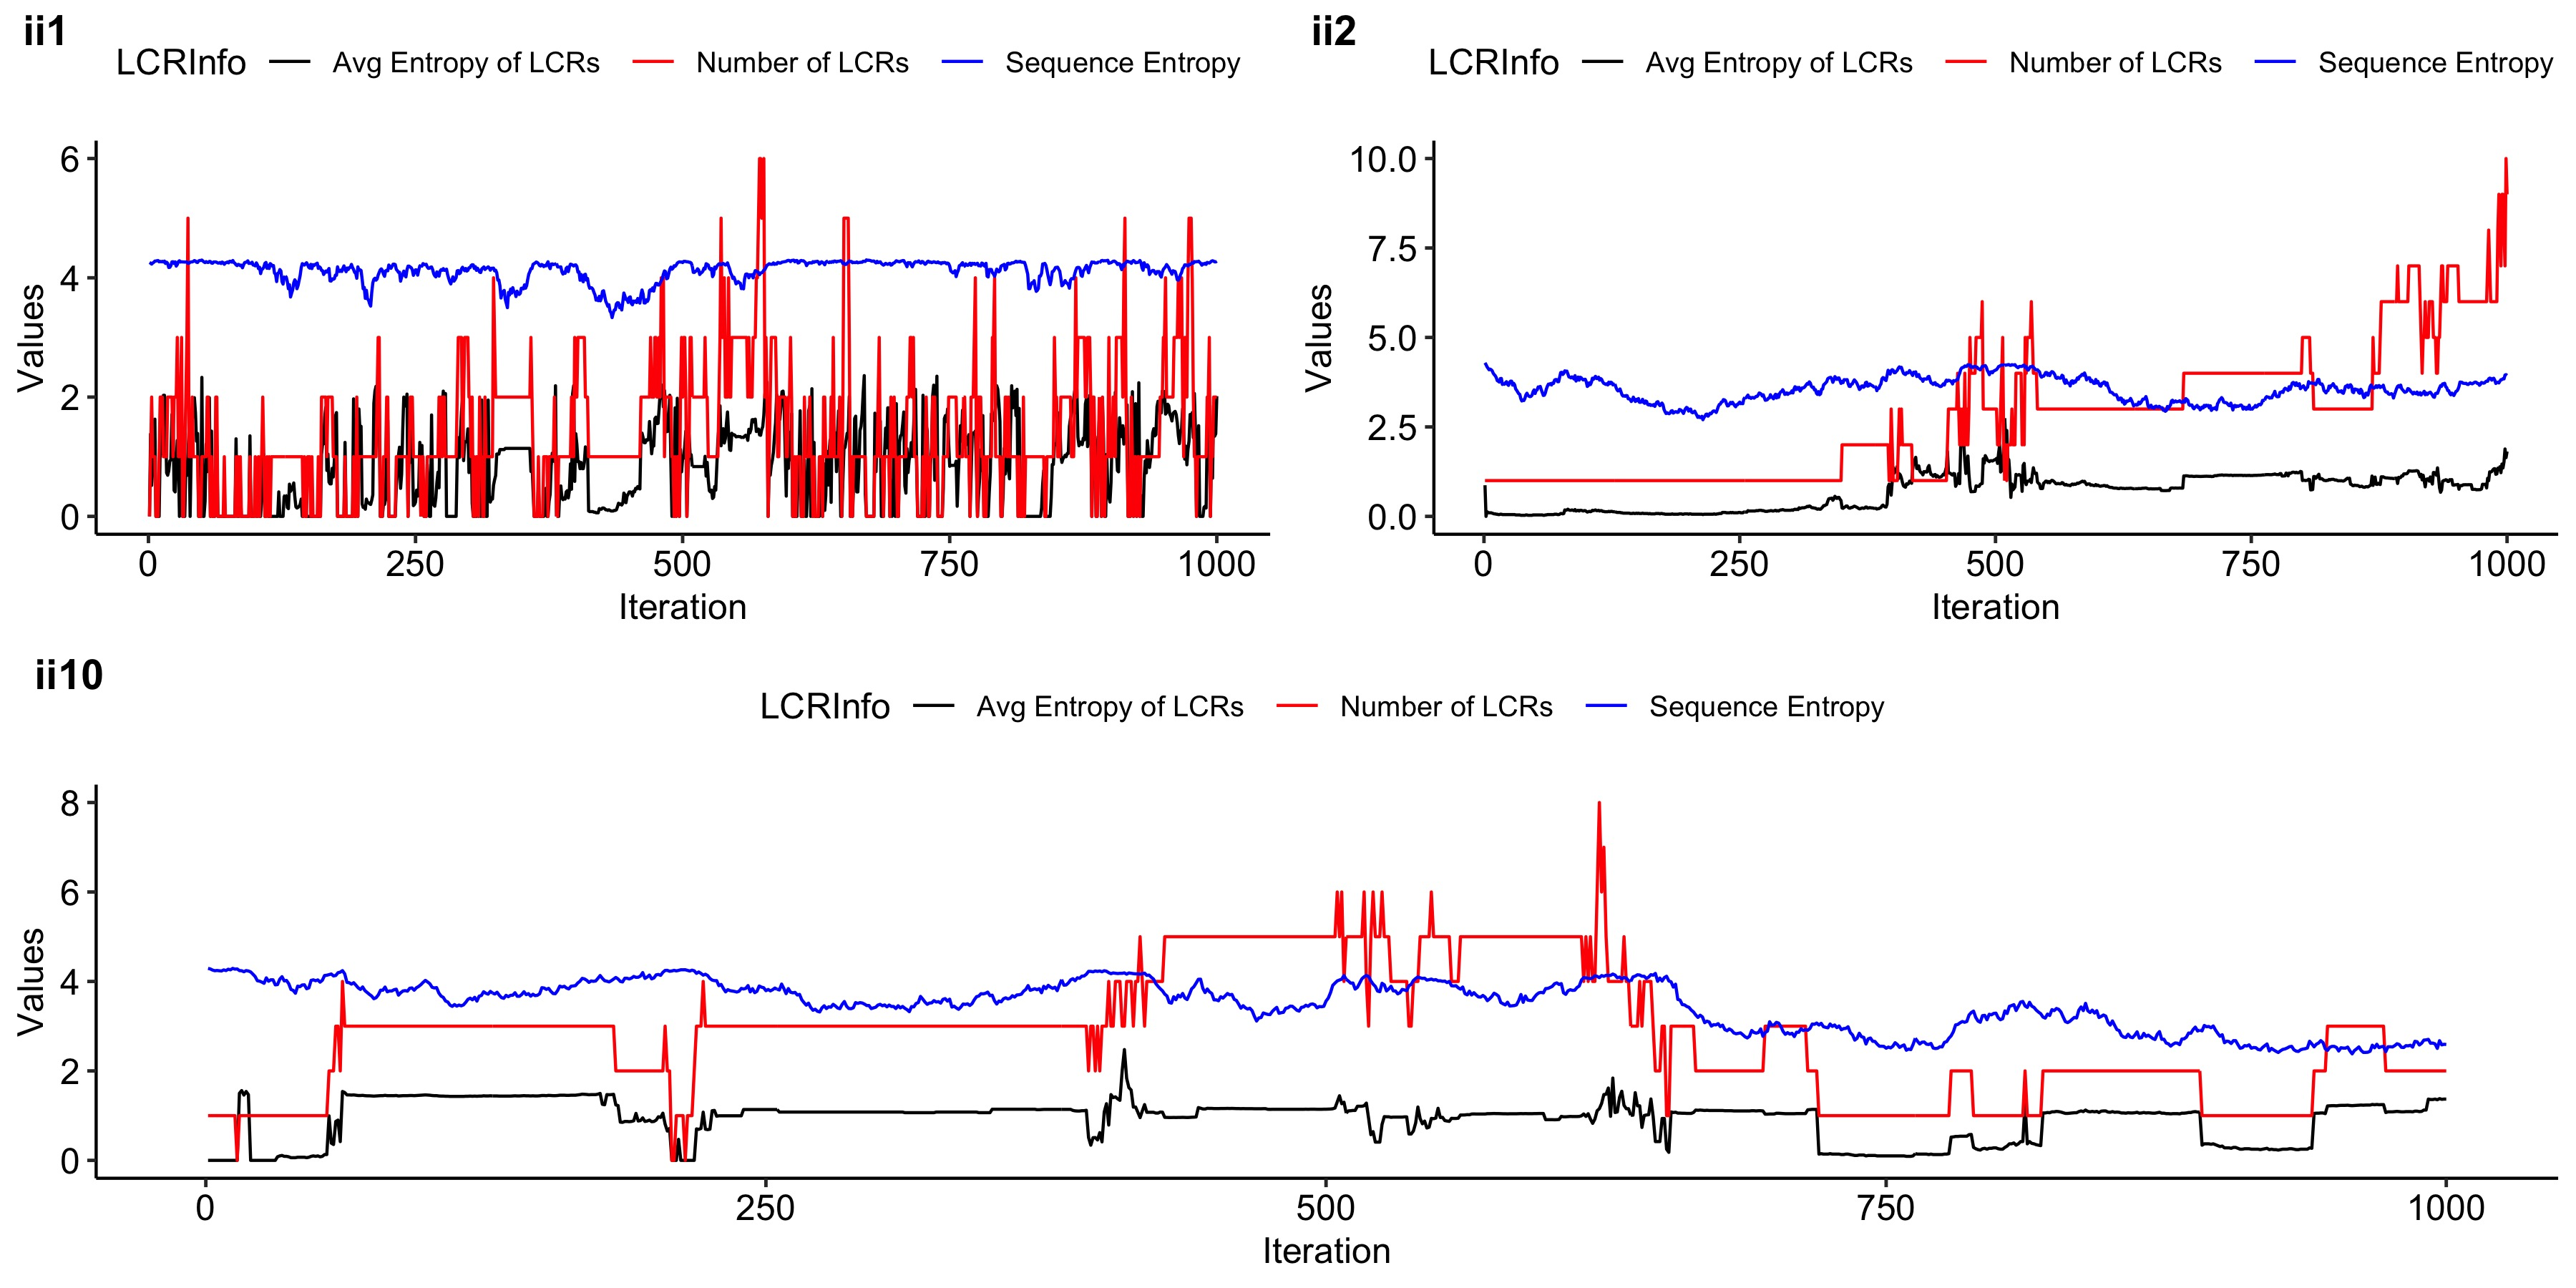
\includegraphics[width=18cm, height=10cm]{im1-2-10.jpeg}
	\caption{Entropy and number of LCR comparisons in a randomly generated protein sequence that has undergone simulated evolution. (TOP LEFT) An indel rate of 1 was utilized. (TOP RIGHT) An indel rate of 2 was utilized. (BOTTOM) An indel rate of 10 was utilized. A mutation rate of 1 was used for all.}
	\label{fig:2}
\end{figure}

To explore the effects of mutation on LCR formation, \figref{fig:3} and \figref{fig:4} show the average sequence entropy, the entropy of the LCRs in the sequence, and the total number of LCRs found in a randomly generated protein sequence that has undergone simulated mutation for 1000 generations. It is expected that under higher rates of mutation, indels will be difficult to form as the large number of mutations destroy repetitive segments. \figref{fig:3} utilized mutation rates of 0.01, 0.1 and 0.5, all of which are less than the fixed indel rate of 1. In all three cases, the average sequence entropy fluctuates as the number of LCRs remains fairly large. In \figref{fig:4}, mutation rates are increased to 1, 2, and 10, much larger than the fixed indel rate. The average sequence entropy fluctuates much less in these cases and the number of LCRs in the sequence decreases in comparison to \figref{fig:3}. These results match the expectation that a larger mutation rate will have major effects of insertions and deletions. In the case where we set the mutation rate to be 10x the indel rate, only three LCRs are formed in total and are quickly removed due to mutation. In this case the entropy is also relatively unaffected, meaning that repetitve regions are not being formed.

It should also be noted that the average entropy of the low complexity regions being formed is significantly less than the average entropy of the entire sequence, and this is expected. 

\begin{figure}[H]
	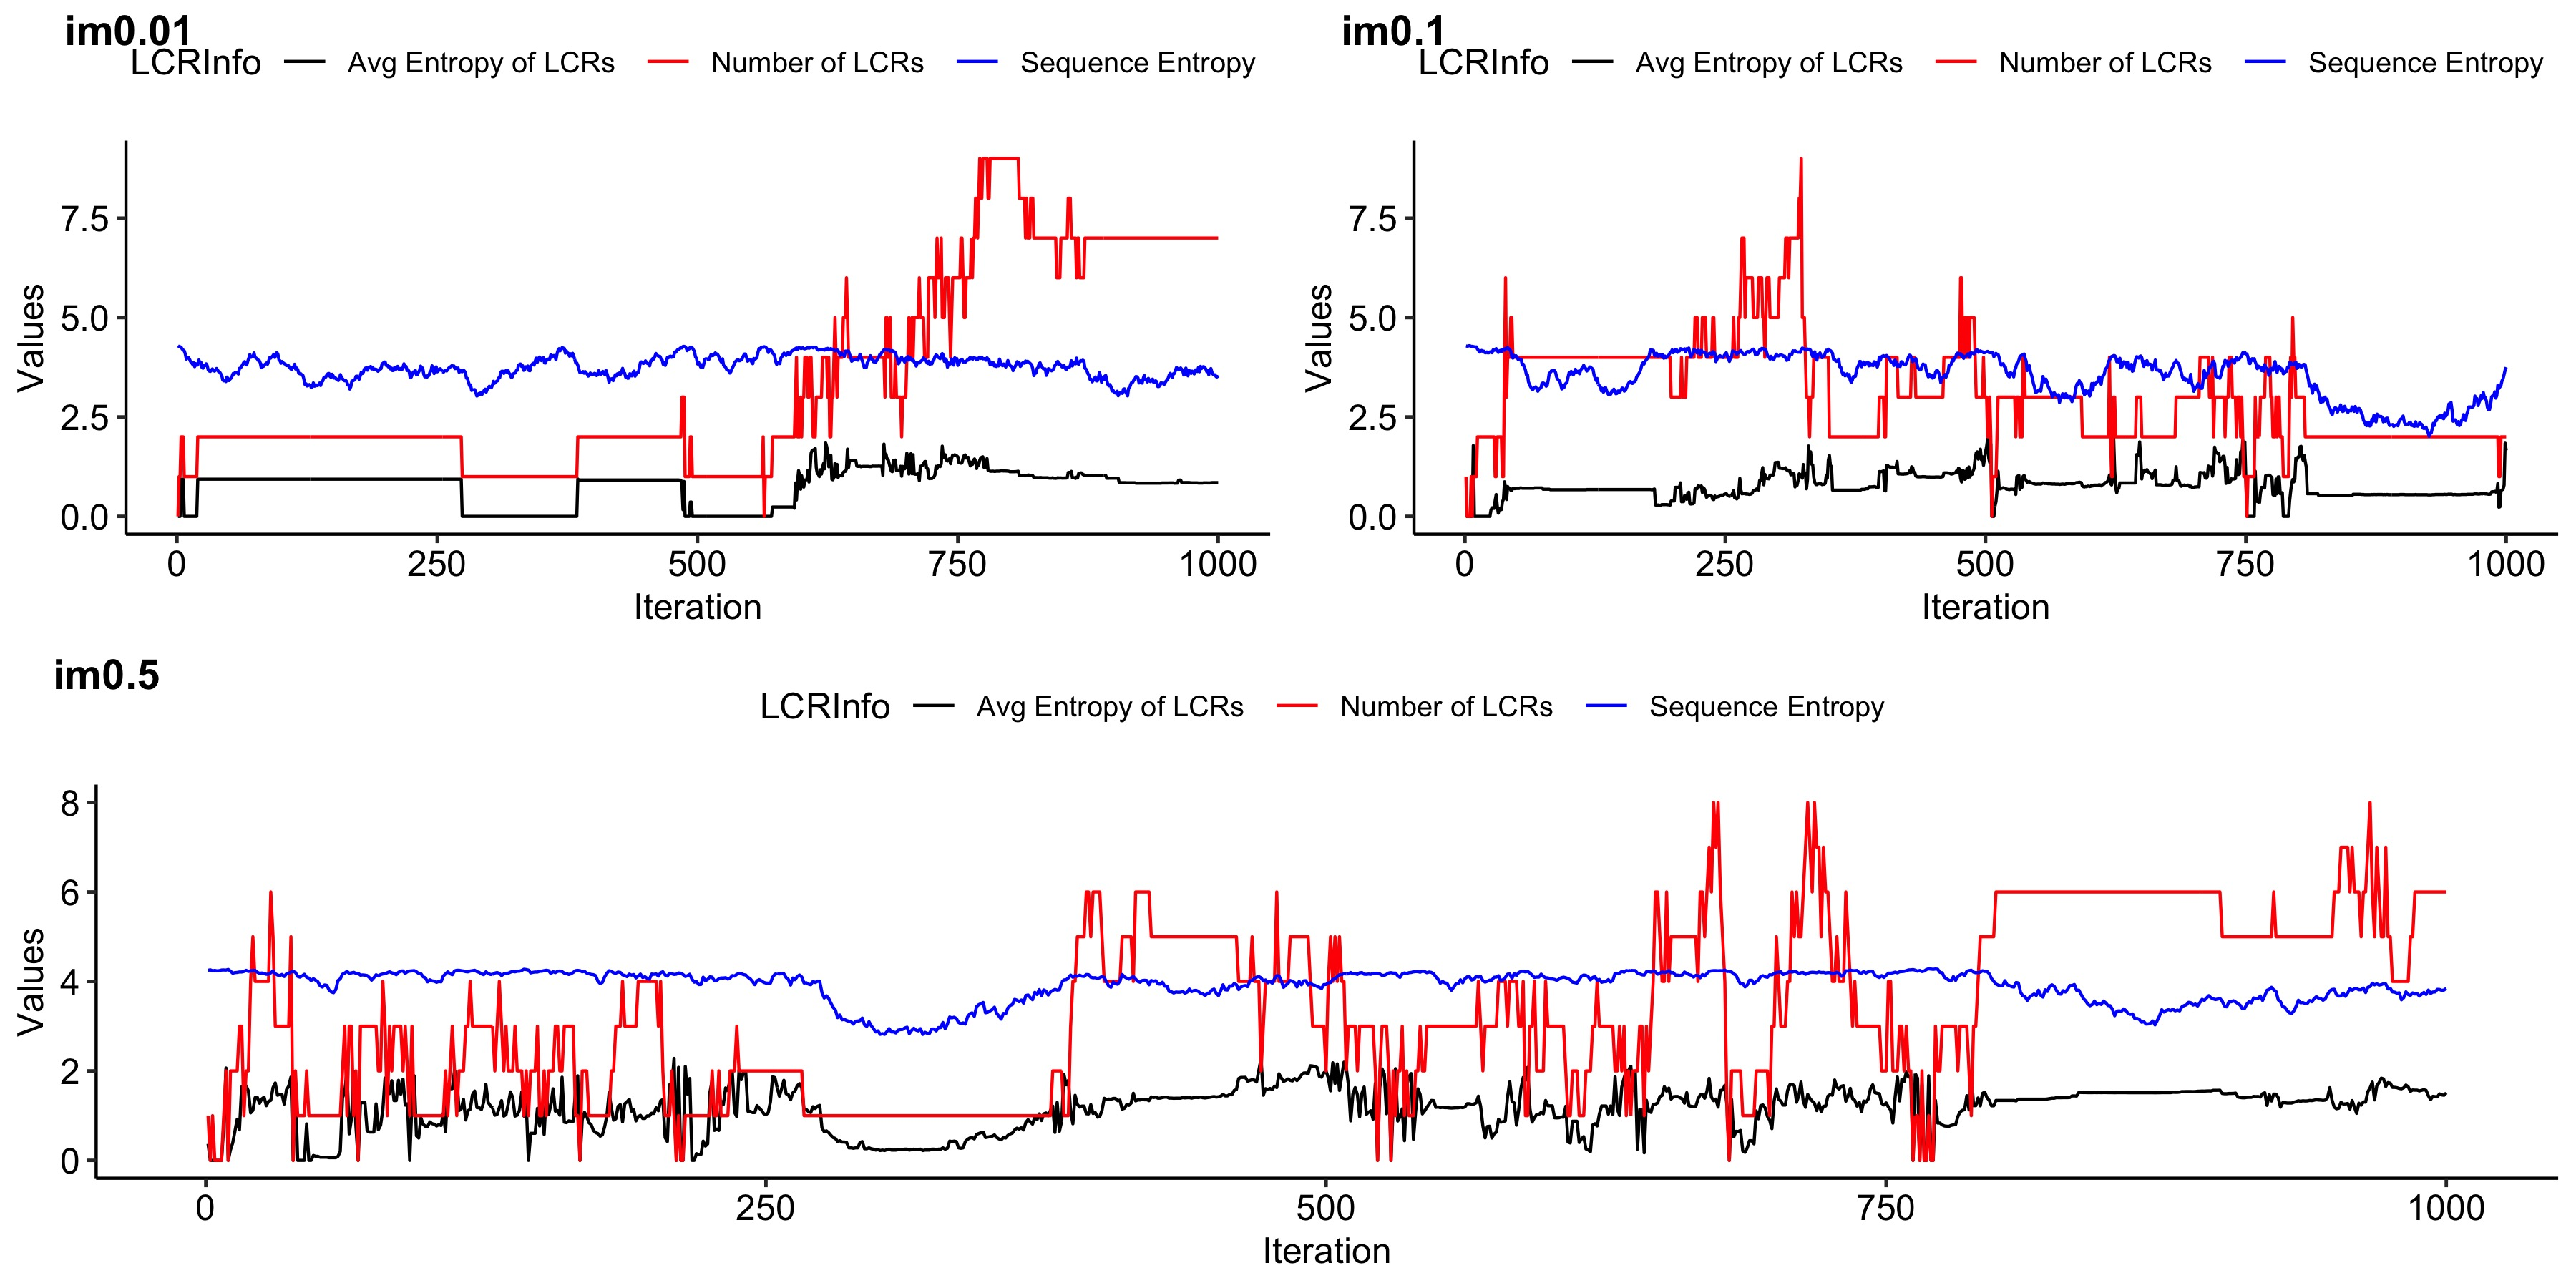
\includegraphics[width=18cm, height=10cm]{m0.01-0.1-0.5.jpeg}
	\caption{Entropy and number of LCR comparisons in a randomly generated protein sequence that has undergone simulated evolution. (TOP LEFT) A mutation rate of 0.01 was utilized. (TOP RIGHT) A mutation rate of 0.1 was utilized. (BOTTOM) A mutation rate of 0.5 was utilized. An indel rate of 1 was used for all.}
	\label{fig:3}
\end{figure}

\begin{figure}[H]
	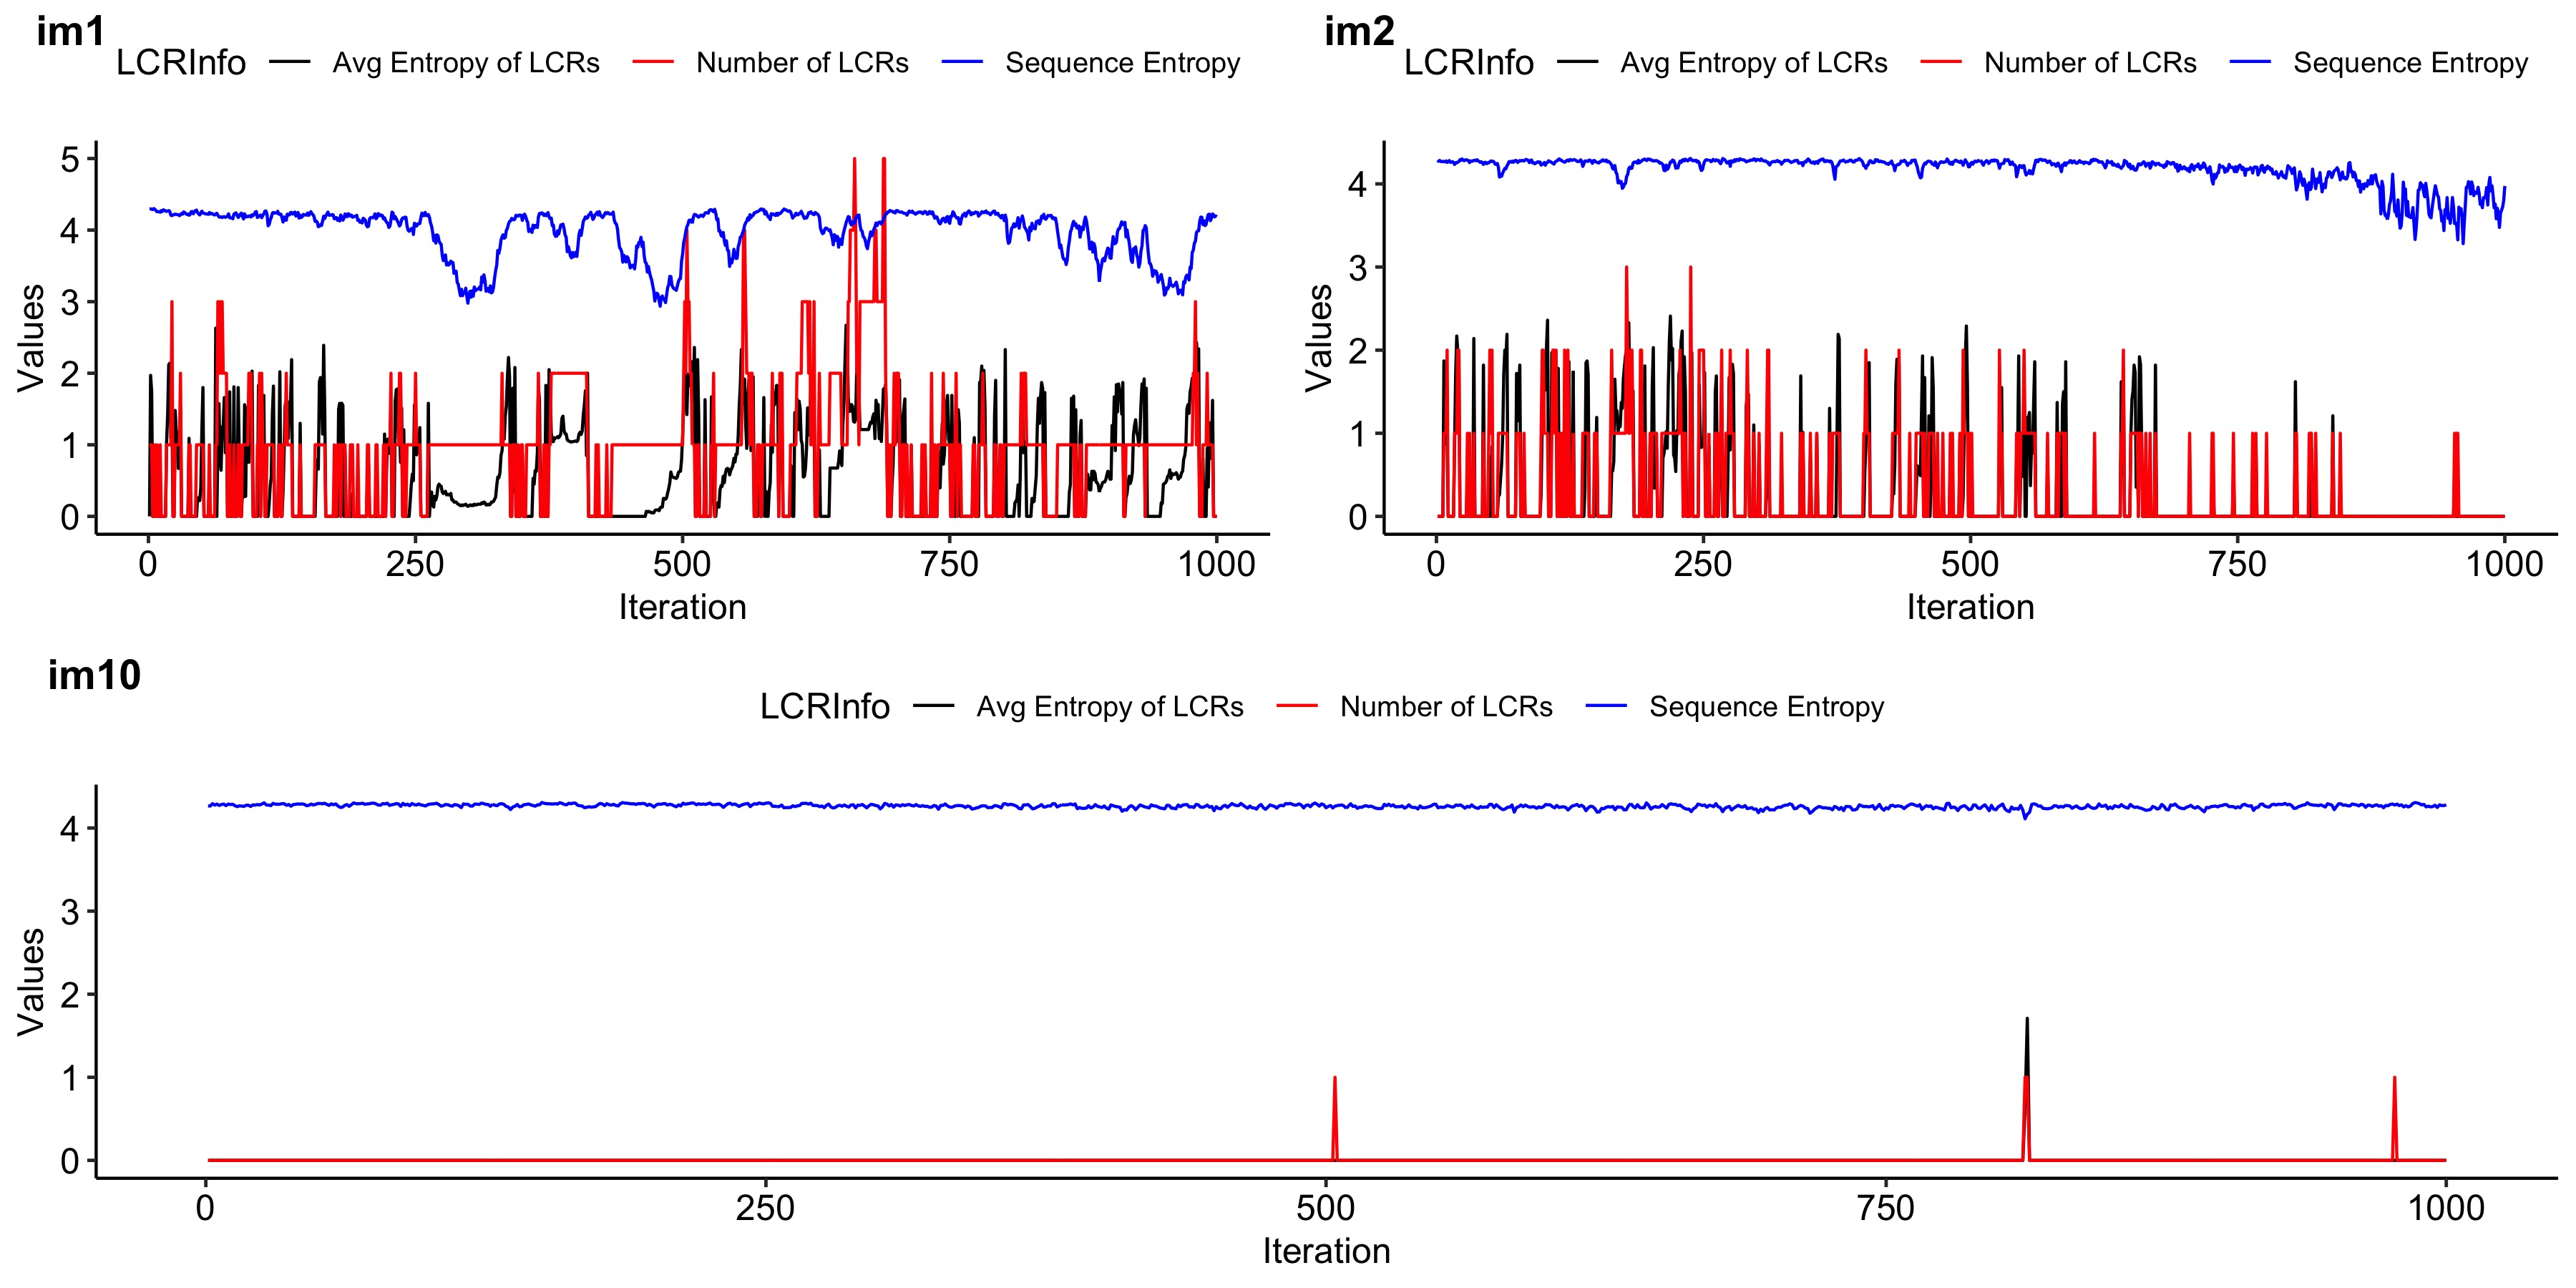
\includegraphics[width=18cm, height=10cm]{m1-2-10.jpeg}
	\caption{Entropy and number of LCR comparisons in a randomly generated protein sequence that has undergone simulated evolution. (TOP LEFT) A mutation rate of 1 was utilized. (TOP RIGHT) A mutation rate of 2 was utilized. (BOTTOM) A mutation rate of 0.5 was utilized. An indel rate of 1 was used for all.}
	\label{fig:4}
\end{figure}


\subsection{Applying the Simulator to an ABC-MCMC}

The second part of this study attempted to create an ABC-MCMC, using the LCR evolution simulator as a step in the algorithm. Time constraints in programming the ABC did not allow for the visualization of posterior distributions. We did however establish that the evolution simulator must be run for a minimum 1000 iterates for each newly proposed parameter value, in order to reach an almost "equilibrium" state. \figref{fig:5} shows the euclidean distance plotted over each iteration of the simulation. The euclidean distance was calculated using vectors of summary statistics for both the simulated protein sequence and the observed protein sequence (SRP40 \scshrt). Essentially the larger the distance, the more differences there are between the simulated protein sequence and the SRP40 protein sequence. In the plot on the left, mutation rate is set to 0 and indel rate is set to 1. In this case, we see the distance between the mutated protein and SRP40 increasing quite rapidly as more LCRs are being formed, and then start to reach a more steady state around 0.5. In the plot on the left, mutation and indel rates are both set to 1. In this case, since mutations are involved as well now, we the distance rapidly increase and start to decrease more steadily at around 0.85.

For each newly proposed parameter value in the ABC-MCMC, we run through the evolution simulator 1000 times and take the average of all 1000 vectors produced. This is why we need to reach some sort of equilibrium in distance to ensure that we reach a level status of both parameters being proposed.

\begin{figure}[H]
	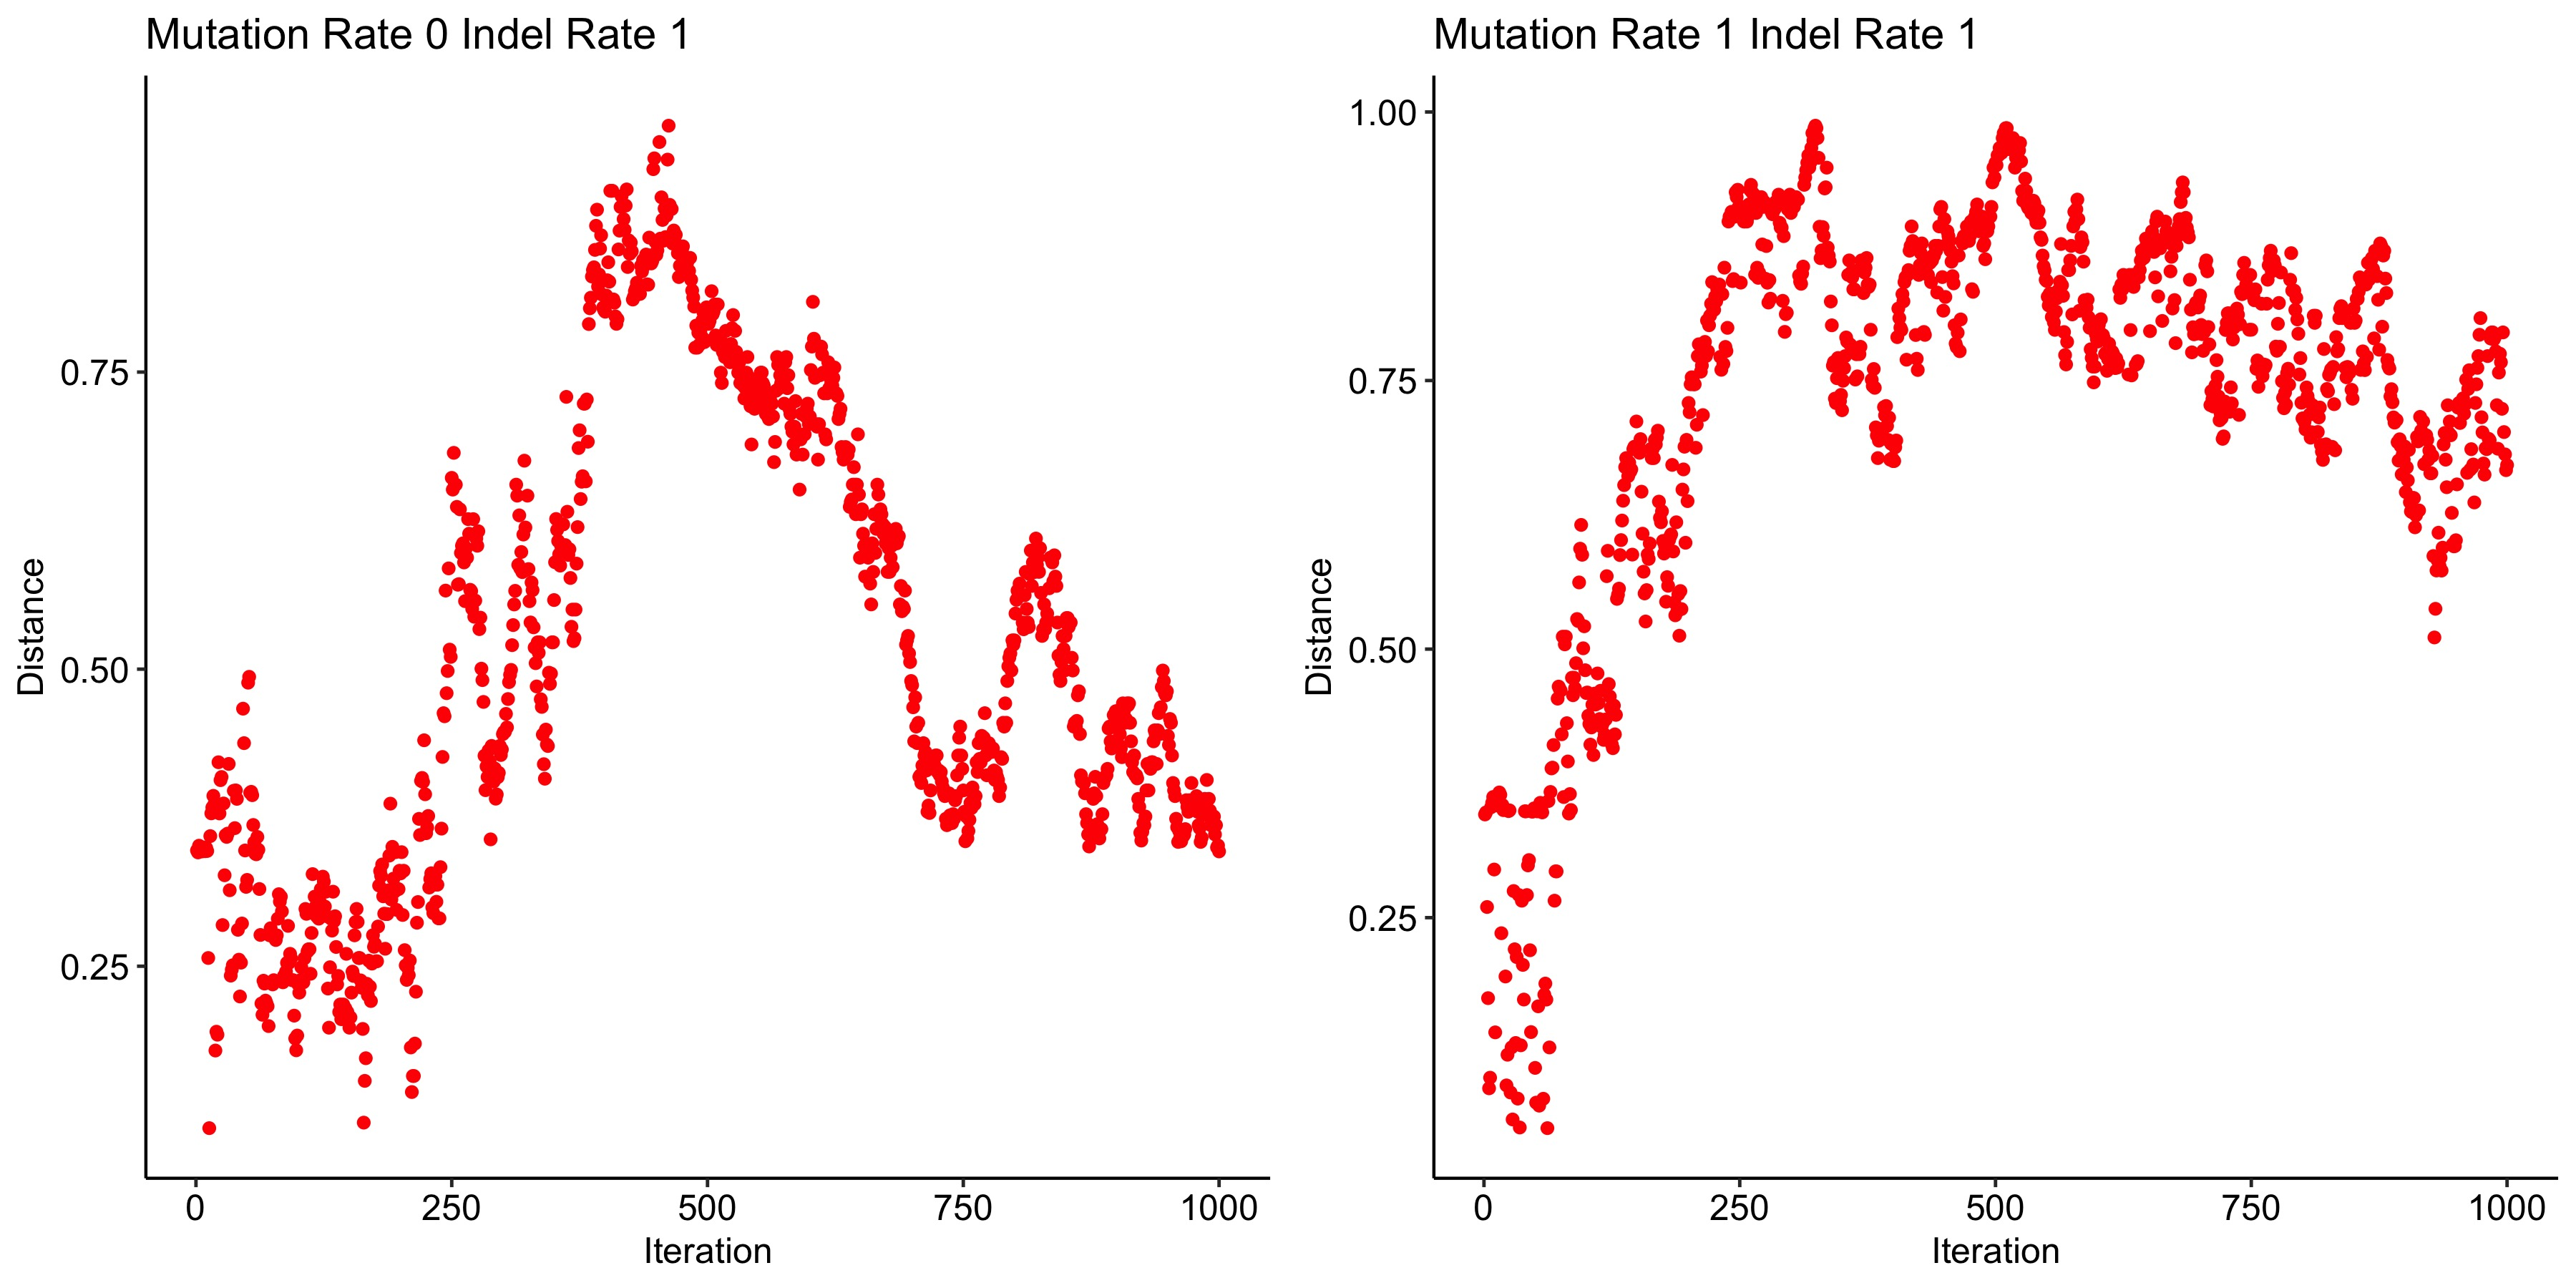
\includegraphics[width=18cm, height=9cm]{distances.jpeg}
	\caption{Calculated euclidean distances between mutated protein and SRP40 protein over 1000 evolution simulator iterates. (LEFT) mutation rate 0, indel rate 1. (RIGHT) mutation rate 1, indel rate 1.}
	\label{fig:5}
\end{figure}
\newpage

\section{Discussion}

This study has developed a method of LCR simulation, which can be used in combination with an approximate bayesian computation markov chain monte carlo method. Due to timing, this study lacks estimates of parameter values that correspond to mutation and indel rates. However, this study does show the benefits of utilizing an approach that does not require calculation of the likelihood function. In the case of this study, mutations, insertions, and deletions alter the landscape of a protein sequence, making it extremely challenging to calculate the likelihood function. In the context of population genetics, ecology, epidemiology and systems biology, ABC approaches have been rapidly gaining popularity due to the massive increase in both the quantity and complexity of biological data \citep{sunnaaker2013approximate}. With the advent of technology and data collection, we are at a point in time where new, tractable approaches must be developed and tested.

\subsection{Mutations Have the Ability to Destroy LCR Formation}

Results obtained from the evolution simulator are heavily dependent on the selected mutation and indel rates. Although both are forms of mutation, each rate parameter corresponds to a different process underneath the hood. Mutation rate in this case refers to the rate at which a base substitution occurs (changing one amino acid into another), while the indel rate refers to the rate at which an insertion or deletion takes place (adding or removing an amino acid residue). By altering mutation and indel rates, we are able to prove the simulation is functioning, and qualitatively assess the effects of having more point mutations on indel formation and vice versa.

With indel rates of 0.1 and 0.5 and a mutation rate of 1, very few low complexity regions are formed, and tend to be destroyed very easily. This is potentially due to the mutation rate being larger, as point mutations have the ability to destroy repetitive regions. As the indel rate is increased to 1,2, and 10, while still holding the mutation rate constant at 1, LCR's are formed in much higher quantities and remain in the sequence for much longer. The overall sequence entropy also decreases with these rates more than the previous rates, due to the increase of low complexity regions contributing to the decrease in sequence entropy. It is interesting to observe that an indel rate 10x larger than the mutation rate does not seem to produce more repetitive, low complexity regions, that swamp out the mutations being created. This could be due in part to the fact that since deletions are also simultaneously occuring, this process could affect how many LCRs are created.

This is not the case however when mutation rates are adjusted and indel rates are held constant at 1. With mutation rates of 0.01, 0.1, and 0.5, many low complexity regions are being formed and the overall sequence entropy tends to fluctuate rapidly. Since the indel rate is higher than the mutation rate in this case, LCRs will be formed and remain stable throughout the entire simulation. When mutation rates are increased to values larger than the indel rates, very few LCRs will be formed and the average sequence entropy will remain close to maximum at about 4.3. With a mutation rate 10x larger than the indel rate, we see the formation of only 3 LCRs which are destroyed in the next iteration, and the average sequence entropy does not fluctuate. This suggests that when the mutation rate is much larger than the indel rate, we are very rarely forming repeats, and when we do, they seem to be immediately destroyed by mutation.


\subsection{Does the Length of a Repeat Play a Role in Insertions/Deletions}

Insertions and deletions (indels) are a very important type of spontaneous mutation, as they make up the majority of the divergence among species \citep{britten2002divergence, anzai2003comparative}. Indels however have been studied much less extensively compared to point mutations \citep{cartwright2009problems}. In this study, deviates were drawn from the exponential distribution and assigned to each individual amino acid residue. When deviates were assigned to residues that were part of a repetitive unit, the length of the repeat was multiplied by the indel rate, and this value was used as the scale parameter ($\beta$) of the exponential distribution. The reason for doing this is because it has been repeatedly observed in both DNA and proteins that the occurrence of indels declines monotonically as a function of their length \citep{pascarella1992analysis, benner1993empirical, qian2001distribution, loewenthal2021probabilistic}. As the length of a repeat increases, so does the scale parameter we use to draw deviates from the exponential distribution. With a larger scale parameter, the mean of the distribution also increases and there is a greater chance we draw deviates with larger values. This subsequently means that the longer the repeat is, the less likely it is to continue to gain repeats and hence we see this monotonic decrease in the occurrence of indels.

This monotonic decrease could also explain why an indel rate 10x larger than the mutation rate does not produce a protein chalked full of repetitive regions. As the indel rate is increased, the number of LCRs increases, but as these LCRs continue to increase in length, it becomes increasingly rare to continue to add repeats in that region. An ideal extension of this research would be to explore alternative relationships which describe the role of the length of a repetitve region in its subsequent mutation. This could be done through assigning deviates for repeats based on different mathematical functions. Currently deviates are assigned to repeated amino acids by multiplying the length of the repeat by the indel rate, but this could be potentially changed to multiplying the indel rate by an exponential function, $e^{length}$. In this case, as the length of the repetitive region increases, the exponential part of the function would also increase exponentially. This means that when we have longer repeats, it will be more difficult to keep adding repeats due to the extremely large scale parameter that would be used to draw deviates from the exponential distribution.

\subsection{Why Parameters Could not be Estimated}

As previously stated, the ABC-MCMC did not produce posterior distributions to estimate parameter values for mutation and indel rates. Overall, the process behind an ABC-MCMC is very complex, but in this study we simplified many of the steps in the algorithm, which could potentially be the reason posterior distributions were not produced. 

An area of major concern in this study stemmed from the chosen summary statistics. Summary statistics are vital in order to quantitatively capture relevent information about the data under analysis \citep{sunnaaker2013approximate}. One potential issue with the summary statistics is that they could not be explaining the characteristics we want in the best way. In this study, we utilized the average number of LCRs, the average entropy of those LCRs, and the length of the entire protein sequence as characteristics that explained the protein sequence. These summary statistics may be too general to accurately capture the differences between a protein of known low complexity (SRP40 \scshrt), and a randomly simulated protein sequence. The goal of the ABC-MCMC was to essentially simulate a protein similar to a known protein sequence using various mutation and indel rates, in order to estimate the rates that produce the known sequence. The way this simulated sequence is compared to the known sequence is only through these summary statistics, not by the composition of the sequence itself. This means for example that a simulated protein sequence could have 3 LCRs (Same as in SRP40), but these LCRs could be in different locations and made up of different amino acids, which means the simulated protein is still very different from the known protein, but we are inccurately saying they are similar based on this summary statistic.

It could also be the case however that the summary statistics used in this study required specific weightings to minimize certain statistics from dominating the distance calculation. The length summary statistic tended to be a dominating force when running the ABC, which affected how often we accepted and rejected parameter values. Due to the fact that we attempted to estimate two parameters with the ABC, it is often the case that while a statistic may estimate one of these parameters well, it may not do the same for the other \citep{hamilton2005bayesian}. A potential workaround for this is to implement a weighting scheme that essentially gives greater weights to statistics carrying more information on the parameter of interest \citep{hamilton2005bayesian}. The way this could be done is to assess relationships between parameters and statistics using local regressions, and subsequently implement a weighted Euclidean distance using the results from the local regression. \citep{hamilton2005bayesian}. Through multiplying summary statistics by a certain weight, it could potentially allow for the acceptance of more parameters due to statistics like length not being the dominating factor in the Euclidean distance calculation.

\subsection{Conclusion}

In summary, the creation of a program that simulates the evolution of low complexity regions can enable the exploration of new model based approaches such as approximate bayesian computations. This can subsequently allow for predictions to be made regarding the evolutionary history of protein or DNA sequences. This research also contributes to the lack of knowledge there is surrounding indels and the way in which they evolve. Through adjusting models of indel evolution using the simulator, the way in which indels are formed can be better understood. This research provides the ground work that is required for utilizing approximate bayesian computation approaches in the context of low complexity regions. The evolution of low complexity regions is still a growing area of research, as the complexity behind how they evolve makes it very difficult to analyze the way they evolve. This research can help pave the way for future work into using model based analyses for exploring the evolutionary dynamics of low complexity regions in proteins.

\clearpage\newpage
\section{References}

%%%FIGURES%%%%%

%%%%PRINTING BIBLIOGRAPHY%%%%
\nocite{*}
\printbibliography[heading=none, sorting=nyt]
\newpage

The following files included these appendices are located at \texttt{/home/alext/scratch/abcmcmc-thesis4c12}

\section{Appendix 1: Low Complexity Region Evolution Simulator}
\texttt{/home/alext/scratch/abcmcmc-thesis4c12/mutations\_2\_BG\_vecs.cpp}
\lstinputlisting[language=c++]{../mutations_2_BG_vecs.cpp}
\newpage

\section{Appendix 2: ABC-MCMC in C++}
\texttt{/home/alext/scratch/abcmcmc-thesis4c12/abcmcmc.cpp}
\lstinputlisting[language=c++]{../abcmcmc.cpp}
\newpage

\section{Appendix 3: Simulated Protein Summary Statistics}
\texttt{/home/alext/scratch/abcmcmc-thesis4c12/abcmcmc.cpp/simulated\_protein.cpp}
\lstinputlisting[language=c++]{../simulated_protein.cpp}
\newpage

\section{Appendix 4: Euclidean Distance and Normlization of Vectors}
\texttt{/home/alext/scratch/abcmcmc-thesis4c12/abcmcmc.cpp/distance2.cpp}
\lstinputlisting[language=c++]{../distance2.cpp}
\newpage

\section{Appendix 5: One Sample t-test}
\texttt{/home/alext/scratch/abcmcmc-thesis4c12/abcmcmc.cpp/ttest.cpp}
\lstinputlisting[language=c++]{../ttest.cpp}
\newpage

\end{document}



